\subsection{Utilizando observaciones visuales del ambiente}

Este último experimento es sobre una configuración donde el agente 
tiene acceso a imágenes como observaciones. A diferencia de las
configuraciones experimentales anteriores, aquí se tiene un solo conjunto
de resultados sobre un ambiente continuo y determinista. Sin embargo, 
se pueden muestra que los alcances del método propuesto son prometedores.

\subsubsection{Configuración experimental}

\begin{itemize}
    \item Los elementos del espacio de estados $\mathcal{S}$, son continuos.
    Las observaciones son imágenes de $84\times 84$ pixeles en un espacio de color RGB, obtenidas desde una vista cenital del ambiente.
    
    \begin{figure}[H]
        \centering
        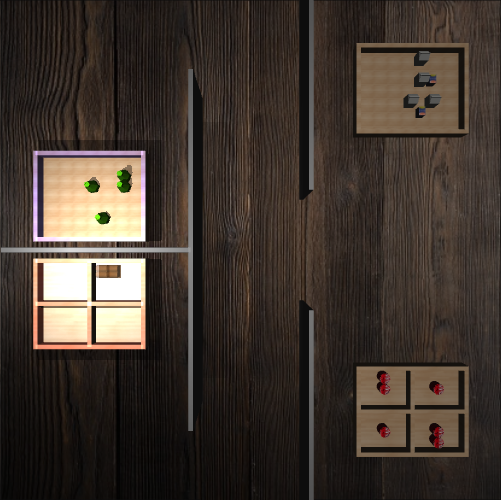
\includegraphics[scale=0.2]{Chapter5/Figs/obs_example.png}
        \caption{Ejemplo de una posible observación del agente.}
        \label{fig:obs-example-lights}
    \end{figure}
    \item Para mapear las imágenes al espacio de estados de alto nivel $\mathcal{X}$, la función $\phi$ es un clasificador multi etiqueta
    parametrizado por una red neuronal convolucional \cite{Goodfellow-et-al-2016} (CNN por sus siglas en inglés). La arquitectura de la red, de manera visual, se presenta en la Figura \ref{fig:cnn-classifier}. Al agente se le brinda el clasificador ya entrenado.
    La salida de la red son procesadores $p_i$ que
    representan la probabilidad de que la variable $x_i$ tome el valor 1, donde
    $i \in \{1, \dots, l\}$. Por simplicidad se utiliza un solo
    clasificador para los distintos experimentos. Por lo tanto, $l = 9$ y
    para los casos donde $N < 9$ entonces se suponen las variables mayores
    a $N$ como apagadas. 
    \item Las transiciones entre estados son deterministas.
    \item El valor de parámetro de alteración del grafo causal correcto es
    $p_{mod} = 25$.
    \item La tasa de decremento de $\epsilon$ está controlada por el factor $\delta = 0.75$.
    \item Dado que las observaciones son imágenes, se utiliza la versión 
    del algoritmo Q-learning para estados continuos DQN. La arquitectura e hiperparámetros de entrenamiento son los mismos que los del artículo original del método DQN 
    \cite{mnih2015human}. 
    
\begin{figure}
    \centering
    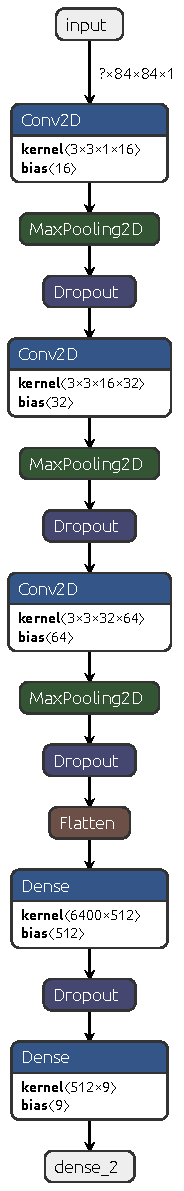
\includegraphics[scale=0.8]{Chapter5/Figs/multilabel_classifier.pdf}
    \caption{Arquitectura del clasificador multi etiqueta, $\phi$, que
    mapea observaciones visuales a un conjunto de variables
    de alto nivel.}
    \label{fig:cnn-classifier}
\end{figure}
\end{itemize}
\subsubsection{Objetivo}

Determinar si el modelo causal con variables  en otro espacio siguen conservando las propiedades
de ayudar en el aprendizaje como en los casos discretos.

\subsubsection{Hipótesis}

Si se cuenta con información de las observaciones
en un espacio más pequeño, pero donde se codifiquen
los estados en alto nivel, se puede apoyar 
al algoritmo de aprendizaje a alcanzar una recompensa
mayor en menos tiempo.

\subsubsection{Resultados}

De acuerdo con la Figura \ref{fig:dqn-results} los algoritmos que utilizan conocimiento del grafo inician con una recompensa mayor y se estabilizan más rápido que el algoritmo DQN
sin información adicional en ambientes con transiciones deterministas. A pesar de que 
el número de episodios
es menor que en el caso 
discreto, parecen mantenerse los mismos resultados 
que en la configuración de un ambiente con observaciones
discretas.

\begin{figure}
\settoheight{\tempdima}{\includegraphics[width=.32\linewidth]{example-image-a}}%
\centering\begin{tabular}{@{}c@{ }c@{ }c@{ }c@{}}
&\textbf{Uno-a-uno} & \textbf{Causa común} & \textbf{Efecto común} \\
\rowname{$N = 5$}&
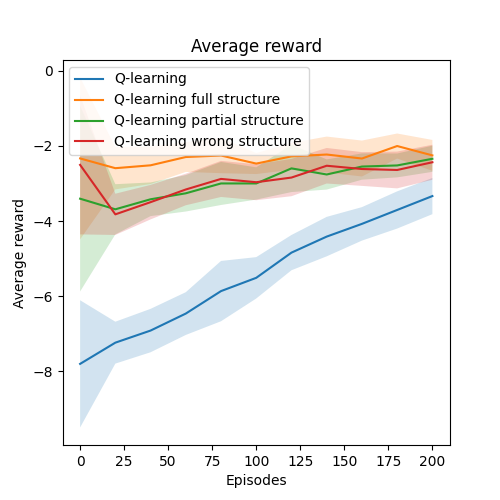
\includegraphics[width=.32\linewidth]{Chapter5/Figs/dqn_plots/comparison_dqn_20_5_one_to_one_200_det.png}&
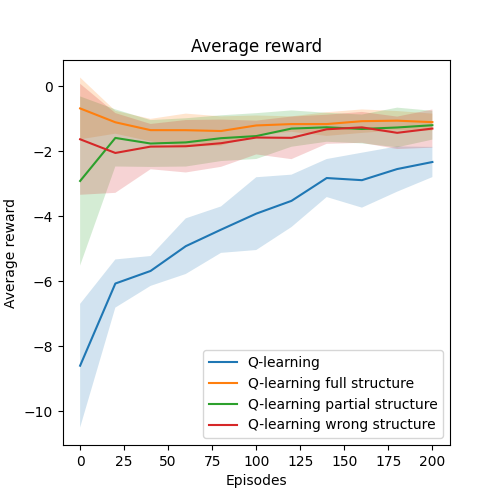
\includegraphics[width=.32\linewidth]{Chapter5/Figs/dqn_plots/comparison_dqn_20_5_one_to_many_200_det.png}&
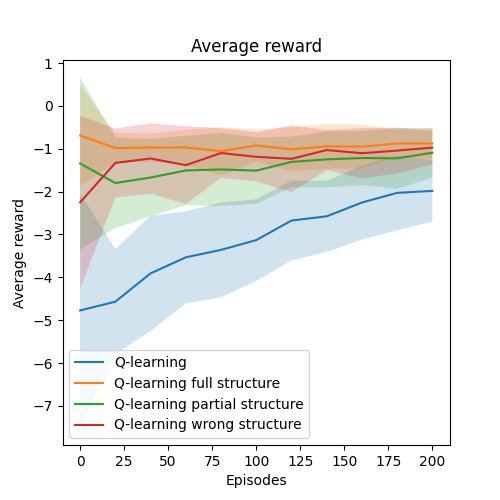
\includegraphics[width=.32\linewidth]{Chapter5/Figs/dqn_plots/comparison_dqn_20_5_many_to_one_200_det.png}\\
\rowname{$N=7$}&
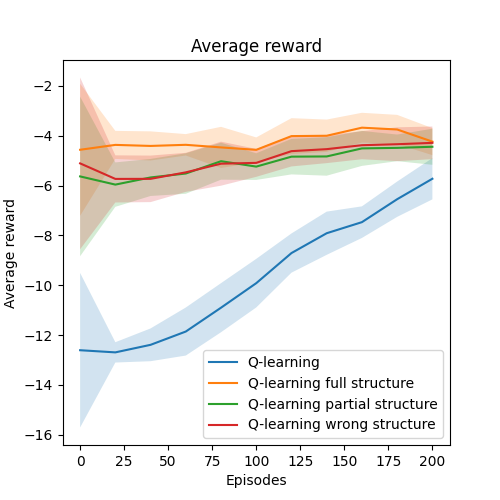
\includegraphics[width=.32\linewidth]{Chapter5/Figs/dqn_plots/comparison_dqn_20_7_one_to_one_200_det.png}&
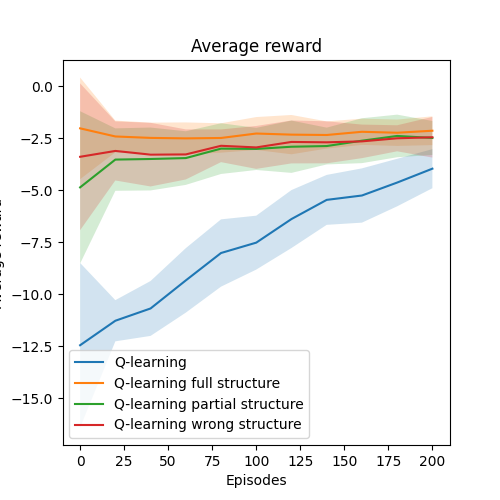
\includegraphics[width=.32\linewidth]{Chapter5/Figs/dqn_plots/comparison_dqn_20_7_one_to_many_200_det.png}&
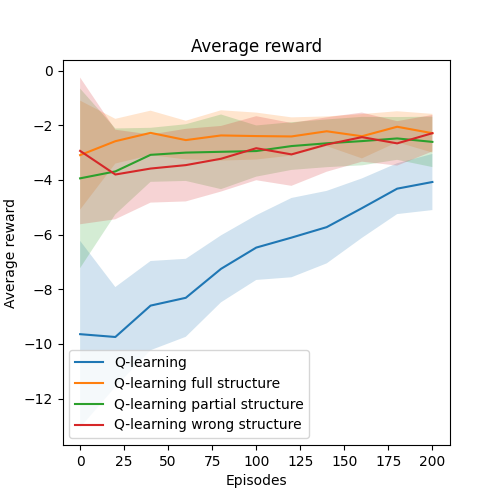
\includegraphics[width=.32\linewidth]{Chapter5/Figs/dqn_plots/comparison_dqn_20_7_many_to_one_200_det.png}\\
\rowname{$N = 9$}&
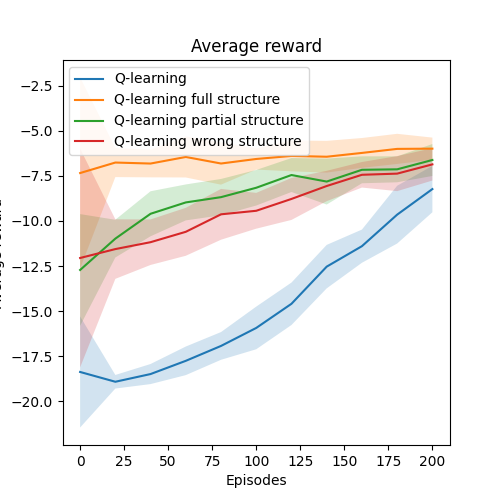
\includegraphics[width=.32\linewidth]{Chapter5/Figs/dqn_plots/comparison_dqn_20_9_one_to_one_200_det.png}&
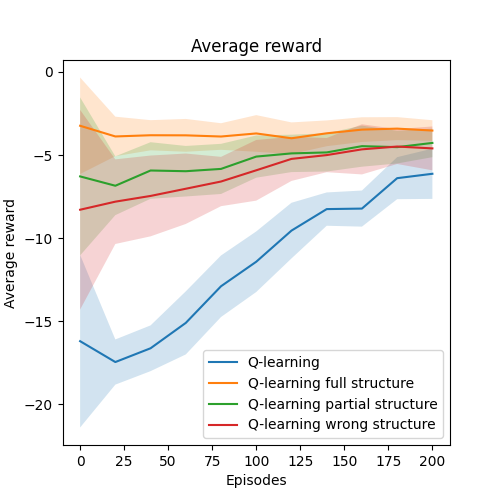
\includegraphics[width=.32\linewidth]{Chapter5/Figs/dqn_plots/comparison_dqn_20_9_one_to_many_200_det.png}&
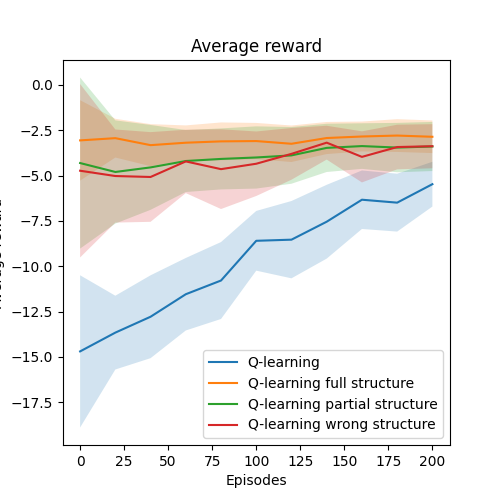
\includegraphics[width=.32\linewidth]{Chapter5/Figs/dqn_plots/comparison_dqn_20_9_many_to_one_200_det.png}

\end{tabular}
\caption{Comparación del desempeño para los 4 algoritmos con $p_{mod} = 25 \%$ y $\delta = 75$ en un ambiente determinista y continuo. Las gráficas muestran la medida $average$ y la desviación estándar (región sombreada) para 10 experimentos con 200 episodios}
\label{fig:dqn-results}
\end{figure}

\newpage
